\section{Motivation and Prior Work}
\label{Background}

In this section we discussed the most closely related work to our proposed technique. Other relevant work will be discussed throughout the paper. See section \ref{related}.

	The idea of prefetching has been around ever since Jouppi introduced \textit{instruction stream buffers}. Early prefetchers detected stride access patterns in order to predict future memory requests ~\cite{Smith,Baer,Stride}. These days prefetching mechanisms are more sophisticated, they look into past memory behavior~\cite{Address_Correlated,AMPM}, locality ~\cite{Spatial_Pattern,SMS,Temporal_Instruction_Fetch,Off_Chip,STMS,SMS_JILP}, control-flow speculation ~\cite{BFetch,MTBFetch}, between many other aspects in order to detect complex access patterns in modern applications.

\subsection{Lookahead-based Prefetchers}

An optimal prefetcher should be able to detect a wide range of memory access patterns. Simple stride prefetching techniques only detect sequences of addresses that differ by a constant value and fail to capture diverse delta patterns. Lookahead prefetchers learn patterns by collecting histories of observed data access patterns, and correlating these with the strides, by considering each new page in a vacumm. Kim textit{et. al.} proposed SPP ~\cite{SPP}, a confidence-based lookahead prefetcher. SPP creates a signature associated to a memory request by compressing the history of accesses. By correlating the signature with future likely delta patterns, SPP learn both simple and complicated memory access patterns quickly. Our proposed technique builds upon SPP, therefore, we now introduce SPP in more detail.  


\subsection{Baseline Prefetcher: The Signature Path Prefetcher}
\label{Background-SPP}

While the basic idea of perceptron based prefetch filtering is applicable to
any look-ahead prefetcher, we developed a practical implementation of the idea
using SPP as our baseline.  Here we describe the basic architecture of SPP.

% djimenez: Paul, is all this stuff accurate? SPP continues to confuse me.

\textbf{Signature Table:} The Signature Table keeps track of 256 most recently accessed
pages.  It is meant to capture memory access patterns within a page
boundary.  SPP indexes into an entry of the Signature Table using the page number.  For
each entry corresponding to a page, the table stores a `last block offset'
and an `old signature'.  Last block offset is the block offset of the
last memory access of that given page.  The block offset is calculated
with respect to the page boundary.  The signature is a 12-bit
compressed representation of the past few memory accesses for that
page.  The signature is calculated as:
$$New Signature = (\,Old Signature << 3 bits\,) \;\;XOR\;\; (\,Delta\,)$$ 
Delta is the numerical difference between the block offset of the 
current and the previous memory access. In case a matching page entry 
is found, the stored signature retrieved and used to index into the 
Pattern Table. This process is illustrated by figure \ref{fig:spp_update}.

\textbf{Pattern Table:} The Pattern Table is indexed by the signature generated
from the Signature Table.  Pattern Table holds predicted delta patterns and their confidence
estimates.  Each entry indexed by the signature holds up to 4 unique
delta predictions.  This is implemented by making the Pattern Table as a 4-way
associative table.

% djimenez: it does look like we're pushing it with all the stuff about SPP.
% Let's describe it enough to give the reader the idea that he/she has a vague
% understanding of how it works and can refer to the MICRO paper for more
% details. (I'm not saying cut anything that's already there, just don't expand.)

%% NOTE: Can we do away with this example? 
%% If it looks like we are writing too much about SPP
%% EDIT: Decided to reorganize and remove this for now.
%% 	Consider the case that incoming page number 10 with a block offset 3
%% 	finds a match in the ST.  The retrieved pattern signature is 0x30 and
%% 	the Last Offset is 1.  Since now there is the Last Block Offset (1),
%% 	Incoming Block Offset (3), Old Signature (0x30), and New Signature
%% 	calculated as per above equation (0x182), SPP can infer
%% 	non-speculatively that the given pattern of memory accesses (as
%% 	captured in the Old Signature) leads to the particular Delta.  In
%% 	general, Delta is defined as the difference between the prefetch
%% 	suggestion block and the initial block which triggered the prefetch.
%% 	In this case, since SPP is in learning phase, it is defined as the
%% 	difference between the Incoming Block Offset and the Last Block Offset
%% 	(+2 in this case).  This, in turn generates the new memory pattern
%% 	(New Signature).  This newly learned signature pattern and the delta
%% 	is stored in the Pattern Table.

\textbf{Prefetch Table:} The Prefetch Table is a 1024 entry 1-way associative table that
keeps a record of last few entries prefetched.  This proves useful for
updating the prefetcher states if a tracked prefetch leads to a demand hit or
a cache eviction. \textit{Note:} The original paper refers to this as the Prefetch Filter 
but since in our context filter refers to the perceptron filter, we will be calling 
this structure as the Prefetch Table to avoid any confusion.

\textbf{Lookahead Prefetching:} On each trigger, SPP goes down
the program speculation path using its own prefetch suggestion.
Using current prefetch as the baseline, it re-accesses the Pattern Table to generate further
prefetches. It repeats the cycle of accessing Pattern Table and
updating the signature based on highest confidence prefetch from the
last iteration.  The iteration counter on which SPP manages to
predict prefetch entries in the lookahead manner is characterized as
its `depth'.  While doing so, SPP also keeps compounding the
confidence in each depth.  Thus as depth increases, overall confidence
keeps decreasing.  

\textbf{Confidence Tracking}: The Pattern Table keeps a count of hits to each
signature through a counter C\textsubscript{sig}.  The number of hits
for a given delta per signature are tracked using a counter
C\textsubscript{delta}.  The confidence for a given delta is
approximated through C\textsubscript{d} = C\textsubscript{delta} /
C\textsubscript{sig}.  When SPP enters into a lookahead mode, the path
confidence P\textsubscript{d} is given as:
$$P\textsubscript{d} \;=\; \alpha  \;.\;  C\textsubscript{d}  \;.\;  P\textsubscript{d-1}$$ 
Here $\alpha$ represents the global accuracy, calculated as the ratio of 
the number of prefetches which led to a demand hit to the number of 
prefetches recommended in total. The range of $\alpha$ is [0,1].

`D' is the lookahead depth. For $d = 1$, when SPP is in
non-speculative mode, P\textsubscript{0} can be thought of as 1. 
The final P\textsubscript{d} is thresholded against PF\_THRESHOLD 
(T\textsubscript{p}) to reject the low confidence suggestions and 
then against a numerically bigger FILL\_THRESHOLD (T\textsubscript{f}) to 
decide whether the prefetch should be sent to L2 Cache 
(high confidence prefetch) or Last Level Cache (low confidence prefetch).
The two thresholds were empirically set to 25 and 90 respectively, 
on the scale of 0 to 100.  

%<Insert a comprehensive figure about SPP structures>

\begin{figure}
  \begin{center}
  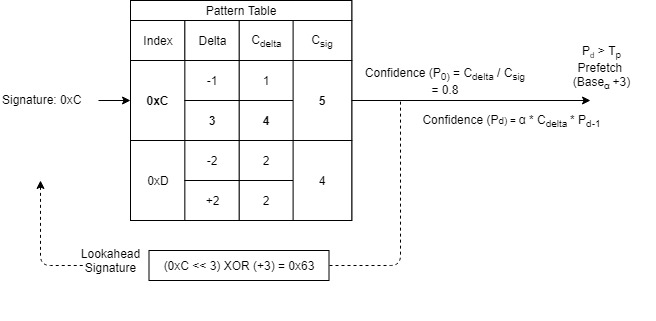
\includegraphics[width=9cm]{figures/SPP_Prefetch_Description.jpg}
    \label{fig:spp_strcture}
  \caption{SPP architecture}
  \end{center}
\end{figure}

%<Insert another detailed picture about SPP data-path flow>
\begin{figure}
  \begin{center}
  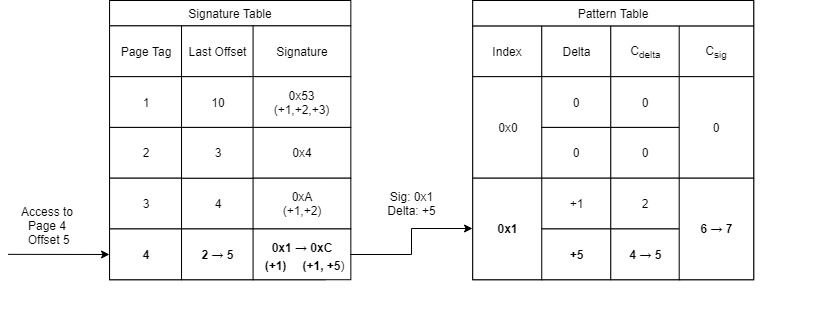
\includegraphics[width=9cm]{figures/SPP_Update_Description.jpg}
  \label{fig:spp_update}
  \caption{SPP data-path flow}
  \end{center}
\end{figure}

% djimenez: this detail is unnecessary and likely to invite questions.
% reviewers might ask "what about linear separability?" but the proof is in the
% pudding.
%This form of indexing makes sure that the hyper-plane learned by the
%perceptron weights is able to differentiate between linearly
%inseparable outcomes. 

%\textit{Deviations From Actual Perceptrons:} Traditionally, a perceptron
%prediction involves multiplying the vector of input features:
%F\textsubscript{1xN}, with the corresponding weight vector:
%W\textsubscript{Nx1} in a dot product to obtain the sum y\textsubscript{out}.
%Here what we use is a perceptron-like structure.  The feature is used to hash
%into the weight of perceptrons and the retrieved weights are added straight
%away.  Thus, the perceptron algorithm doesn't introduce any multiplication
%operations in the inference or training process.  Hence what we adapt in this
%work is a perceptron-like learning algorithm as it involves the same principle
%involved in perceptron inferencing and training.


\subsection{Case for an On-line Filter}
\label{Background-Case}

Compared to some of the other state of the art prefetchers, SPP is
less aggressive.  In a single-core environment, there is no resource
contention among the different cores, hence aggressive prefetching is bound to prove beneficial. 
As we increase the core
count, we observe that SPP starts outperforming rest of the prefetchers.  This
can be attributed to the fact that each prefetch suggested by SPP is a
carefully calculated and prevents cache pollution.  \textit{<Figure
showing the variation of SPP vs BOP wrt core count>} For 4-core applications,
SPP suggests XX\% fewer prefetches than Best Offset Prefetcher ~\cite{bop} and yet leads to higher IPC.

The above analysis shows that with a more careful filtering mechanism, any
prefetcher like SPP can be tuned to become much more aggressive, yielding higher coverage.  The responsibility of maintaining high accuracy now falls on the
independent filter.  To test the hypothesis, we tuned down SPP to the
minimum possible threshold, with the effect of increasing prefetch suggestions
made by SPP by XX\%.  \textit{<Comparison of SPP-Unleased with SPP / BOP>}
Obviously this came at a cost of increased DRAM traffic and cache pollution.

Moreover, the on-line confidence mechanism introduced in SPP was very
rudimentary.  It was based on taking a ratio C\textsubscript{d} =
C\textsubscript{delta} / C\textsubscript{sig} as explained previously. This
confidence was used to make the decision of whether to prefetch or not to
prefetch; and which level to prefetch.  While this approximation was shown to
work in the original implementation, we believe that a better form of
generalised on-line decision making was possible.  Hence, it was necessary to
build a robust and adaptable learning mechanism to accept / reject the
prefetch suggestions; and to decide the fill level (L2 Cache vs Last Level
Cache).

To that effect, we introduce an independent on-line perceptron based
filtering mechanism.

\subsection{Supervised Learning}

\textit{Perceptron Learning Rule:} In a perceptron-based mechanism, a uniform
perceptron update principle is followed.  The weights need to be updated if
the prediction was wrong or the magnitude of the dot product does not exceed
a certain threshold.  After a certain training period, these weights are
proportional to the probability of a correct prediction.  Thresholding the outcome to a
 magnitude makes sure the perceptrons are trained until a certain level of
confidence and yet they are not over-trained to the given set.  The perceptron 
learning rule will be applied to PPF.
